\documentclass[../en-fa-lab.tex]{subfiles}

% !TeX spellcheck = ro_RO
\usepackage{amsmath}
\usepackage{amsfonts}
\usepackage{amssymb}
\usepackage{graphicx}
\usepackage{hyperref}

\hypersetup{
    pdftitle={(EN) L9 - BFS},   % The title shown in the browser tab
    pdfauthor={},         % Your name or organization
    pdfsubject={},   % A brief description
    pdfkeywords={}
}

\begin{document}
\section{\texorpdfstring{\textbf{Assignment No. 9. BFS: Breadth-First Search}}{Assignment No. 9. BFS: Breadth-First Search}}\label{assign9}




\subsection{Introduction}
In this session you are required to implement and analyse BFS (Breadth-First Search), as presented in subsection 22.2 of Introduction to Algorithms by Th. Cormen et al.

\subsection{The structure of the boiler plate code}
You are already provided with several source files:
\begin{itemize}
    \item \texttt{main.cpp} - the main source file, which makes the calls to the implemented functions and provides the visualization code
    \item \texttt{bfs.h} - contains definitions of data structures and functions used in the project
    \item \texttt{bfs.cpp} - will contain the implementations of the required algorithms
    \item \texttt{grid.txt} - the maze which represents the graph for the demo
    \item \texttt{Profiler.h} - the library used for algorithm evaluation and chart generation
\end{itemize}

\textbf{!!!} You should only make changes to \texttt{bfs.cpp}.

For a user-friendly visualization, \texttt{main.cpp} displays an ASCII-like interface, in which the maze (i.e. the graph) is displayed (black cells are free, white cells represent walls).

\subsubsection{Project setup for Windows, with Visual Studio}
\begin{figure}[h]
    \centering
    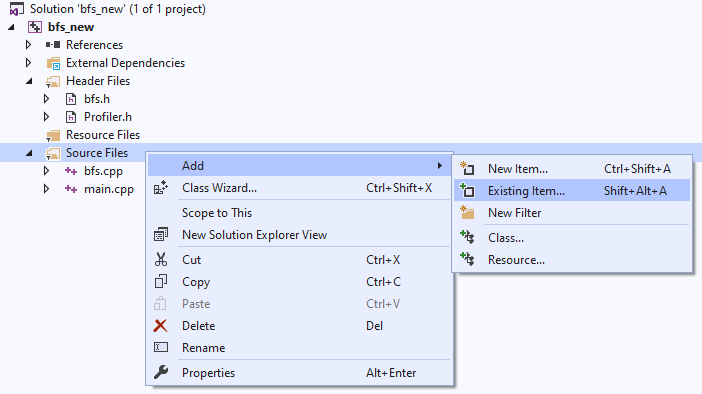
\includegraphics[width=9cm]{../Resources/lab9/vs_solution.png}
    \caption{The \textit{``Solution Explorer''} window in Visual Studio}
    \label{fig:vs}
\end{figure}

Make a new Project in Visual Studio. Make sure to check the \textit{``Empty Project''} checkbox. Then, copy all the files provided in the project folder.

Then, in Visual Studio, add the two files \texttt{.h} to the \textit{``Header Files''} subsection of your project, and the two  \texttt{.cpp} files to the \textit{``Source Files''} subsection (right click on corresponding project subsection  $\rightarrow$ \textit{``Add''} $\rightarrow$ \textit{``Existing Item''}, see Figure~\ref{fig:vs}.

\subsubsection{Project setup for Linux and Mac}
You may edit the source files using your editor of choice. The project comes with a \texttt{Makefile}, so it is enough to run \texttt{make} in a terminal to compile it and generate the executable. The resulting \texttt{.exe} will be called \texttt{main}, and can be run in the terminal by executing \texttt{./main}.

\subsection{Running the program}
When you run the program, it will display the maze, similarly to what you can observe in Figure~\ref{fig:grid1}.

\begin{figure}[h]
    \centering
    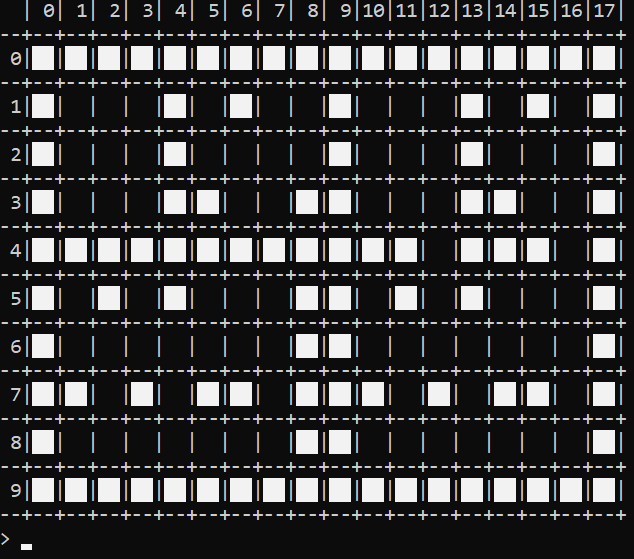
\includegraphics[width=7cm]{../Resources/lab9/grid1.png}
    \caption{Interface of the program}
    \label{fig:grid1}
\end{figure}

The user may input one of the following commands:
\begin{itemize}
    \item \texttt{exit}\\
        program termination
    \item \texttt{clear}\\
        clear the previous information from the grid
    \item \texttt{neighb <row> <col>} \\
        display the neighbors of cell on row \texttt{<row>} and column \texttt{<col>}.
    \item \texttt{bfs <row> <col>} \\
        execute the BFS traversal, starting from the cell on row \texttt{<row>} and column \texttt{<col>}.
    \item \texttt{bfs\_step <row> <col>} \\
        same as \texttt{bfs}, but the result is displayed step by step, depending on the distance from the source node
    \item \texttt{bfs\_tree <row> <col>} \\
        same as \texttt{bfs},  but it will also display the output tree under the grid
    \item \texttt{path <row1> <col1> <row2> <col2>} \\
        displays the shortest path between  \texttt{(<row1> <col1>)} and \texttt{(<row2> <col2>)}
    \item \texttt{perf} \\
        generates the charts for the algorithm evaluation
\end{itemize}

\subsubsection{Example: command \texttt{neighb}}
If you run:\\
\texttt{neighb 2 3}
you should get the output displayed in Figure~\ref{fig:neighb}.

\begin{figure}[h]
    \centering
    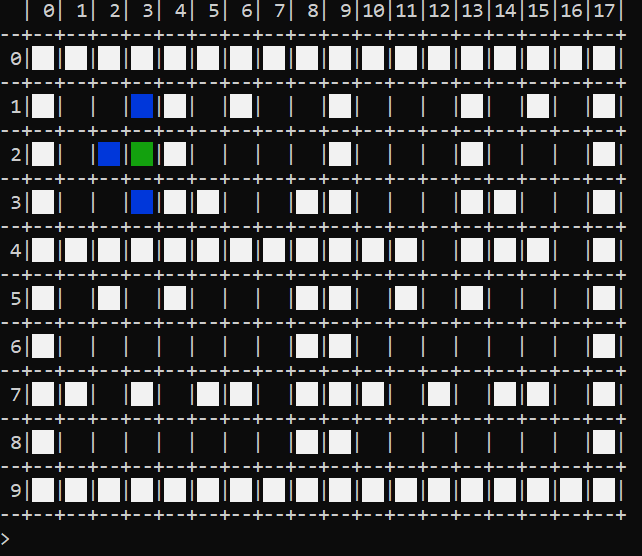
\includegraphics[width=7cm]{../Resources/lab9/grid_neighb.png}
    \caption{The result of running command \texttt{neighb 2 3}}
    \label{fig:neighb}
\end{figure}

The starting cell will be coloured green, with its neighbors coloured blue.

Since \texttt{get\_neighbors()} is not yet implemented (you will be required to do the implementation), you will not get this answer if you run the command. Once you implement the function, you may use this command to check the correctness of your implementation. Each cell can have at most 4 neighbors (up, down, left, right); cells outside the grid or wall cells must not appear as neighbors.

\subsubsection{Example: commands \texttt{bfs} and \texttt{bfs\_step}}
Upon running the command:\\
\texttt{bfs 6 3}
the program should output the result shown in Figure~\ref{fig:bfs1}.

\begin{figure}[h]
    \centering
    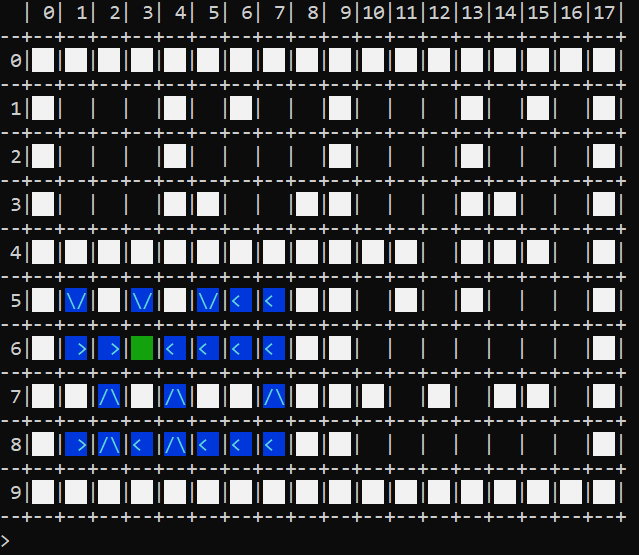
\includegraphics[width=7cm]{../Resources/lab9/grid_bfs1.png}
    \caption{The result of running command \texttt{bfs 6 3}}
    \label{fig:bfs1}
\end{figure}

The source cell will be coloured green, and the other cells traversed will be coloured blue. Each blue cell will have an arrow on it, indicating the direction of the parent in the BFS tree.

Currently, the \texttt{bfs()} function is not implemented. Once implemented, use this command to check the correctness of your implementation.

\subsubsection{Example: command \texttt{bfs\_tree}}
By running:\\
\texttt{bfs 2 6}
you should get the image in Figure~\ref{fig:bfs_tree}.

\begin{figure}[h]
    \centering
    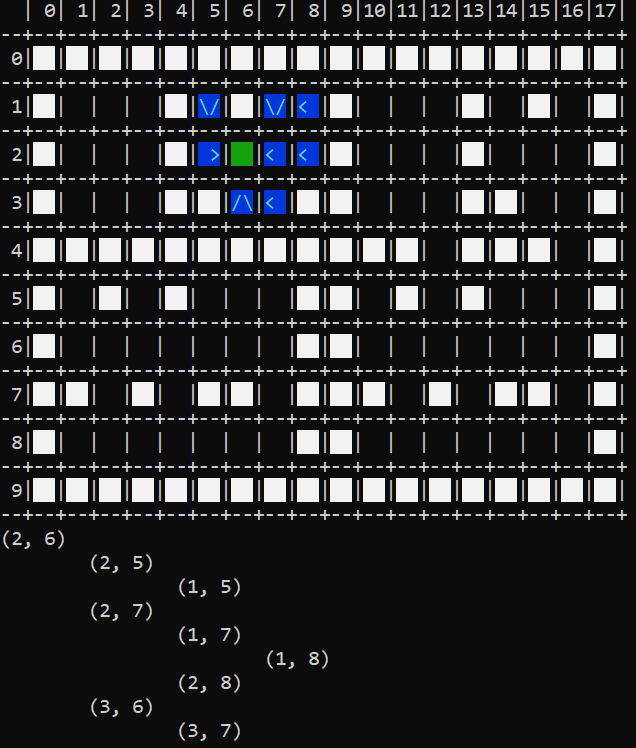
\includegraphics[width=7cm]{../Resources/lab9/grid_bfs_tree.png}
    \caption{The result of running command \texttt{bfs\_tree 2 6}}
    \label{fig:bfs_tree}
\end{figure}

The root of the tree is the source node, i.e. \texttt{(2, 6)}. The children of this node in the tree are: \texttt{(2, 5)}, \texttt{(2, 7)} and \texttt{(3, 6)} (the order might differ, according to the implementation).


\subsubsection{Example: command \texttt{path}}
By running:\\
\texttt{path 5 10 3 15}
you should obtain the image in Figure~\ref{fig:path}.

\begin{figure}[h]
    \centering
    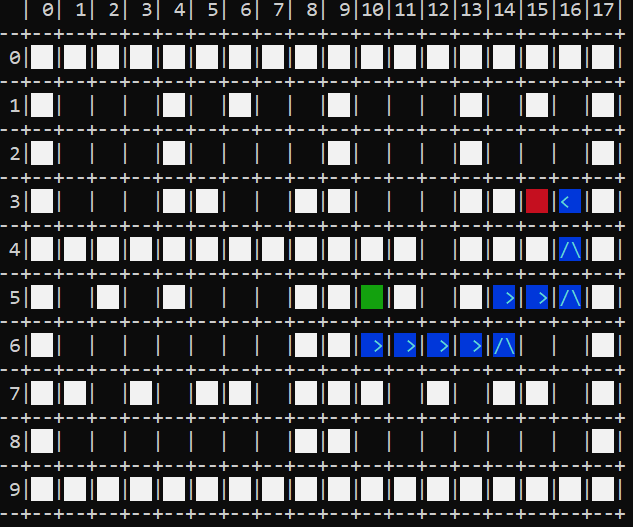
\includegraphics[width=7cm]{../Resources/lab9/grid_path.png}
    \caption{The result of running command \texttt{path 5 10 3 15}}
    \label{fig:path}
\end{figure}

The source cell will be coloured green, the destination cell red, and the rest of the cells on the path - blue. Each blue cell will also have an arrow indicating the direction of the traversal.

Currently, \texttt{shortest\_path()} and \texttt{bfs()} are not implemented, so you will not see this result when running the \texttt{path} command. Once the functions implemented, use this command to check the correctness of your implementations.

\subsubsection{Employed data structures }
The file \texttt{bfs.h} contains definitions of data structures used in the framework.

The \texttt{Grid} structure models a grid, having \texttt{rows} lines and \texttt{cols} columns, the grid elements are stored in the matrix \texttt{mat}. An empty cell has value 0 in the matrix, and a wall cell will have value 1. 

The \texttt{Point} structure models a point (i.e. a grid cell) the \texttt{row} and \texttt{col} fields representing the location, i.e. the row and the column of the point in the grid.

The \texttt{Node} structure models a node in the graph, and it contains:
\begin{itemize}
    \item \texttt{position} having type \texttt{Point} represents the cell corresponding to the graph node.
    \item \texttt{adjSize} - the number of neighbors of the node
    \item \texttt{adj} - the neighbor array, containing \texttt{adjSize} neighbours
    \item \texttt{color} - the color of the node; initially, all nodes are colored \texttt{COLOR\_WHITE}, i.e. the color has value 0
    \item \texttt{dist} -  the distance from the source node, in BFS
    \item \texttt{parent} - pointer to the parent node, in the BFS tree
\end{itemize}

The \texttt{Graph} structure models the graph; it has as members the number of nodes, \texttt{nrNodes} and the array \texttt{v} containing pointers to the neighbor arrays of each node.


\subsection{Requirements}

\subsubsection{Determine the neighbors of a cell (2p)}
In \texttt{bfs.cpp}, tyou have to complete the  \texttt{get\_neighbors()} function which receives
a pointer to a \texttt{Grid} structure, a point \texttt{p} of type \texttt{Point} and an array \texttt{neighb} of
points, which the function will fill with the neighbors of point  \texttt{p}. The function returns the number of neighbors filled in the \texttt{neighb} array.

A point on the grid can have maximum 4 neighbors (up, down, left, right). Not all neighbors are necessarily valid: some may end up outside the grid (negative, or out of bounds coordinates) or inside a wall.Therefore, after computing the position of a potential neighbor, you should check that it is situated inside the grid, on a free value cell (the value in the matrix of the corresponding cell should be 0).

The valid neighbors will be added to the array \texttt{neighb}. It is guaranteed that the array has at most 4 elements, so you may not exceed this capacity. Because the number of neighbors could be less than 4, you should also return this information.

\subsubsection{BFS algorithm implementation (3p)}
In \texttt{bfs.cpp}, you have to complete the function \texttt{bfs()} which receive as arguments a pointer to a structure of type \texttt{Graph} and the source node \texttt{s} of type \texttt{Node*}. The function will implement BFS, as specified in the algorithm from the book (see subsection 22.2 from Cormen).

Initially, the nodes of the graph are colored white, i.e. \texttt{COLOR\_WHITE}, and the \texttt{dist} and \texttt{parent} fields are initialized with 0 and \texttt{NULL}, respectively.  At the end of the traversal, all nodes that can be reached from the cource node are colored \texttt{COLOR\_BLACK}, the distance \texttt{dist} has as value the number of steps from the source node to that node, and the \texttt{parent} pointer should idicate the parent in the BFS
tree.

\subsubsection{Pretty printing the BFS tree (2p)}
In \texttt{bfs.cpp}, t you have to complete the implementation for \texttt{print\_bfs\_tree()} which receives as parameter a pointer to a \texttt{Graph} structure on which the BFS algorithm has already been run, so the node colors and the parent information is already set.

In the function, you already have the construction of the parent array \texttt{p}, in which the nodes colored black in the BFS traversal will be numbered from $0$ to $n$. Also, it builds the \texttt{repr} array, which contains the coordinates of each node (in the grid).

To display this tree, you have to adapt the code from the multiway trees assignment.


\subsubsection{Evaluate the performance of BFS (3p)}
The \texttt{performance()} function evaluates the BFS algorithm, by varying, in turn, the number of edges, then the number of nodes (and always keeping the other as constant). For each value , you have to implement the generation of a random, connected, graph, having a given number of nodes and edges, respectively.

Inside the \texttt{bfs()} function, you will have to actually count the operations performed, using the optional argument \texttt{op}. Because this parameter is optional, sometimes \texttt{bfs()} will be called by the framework with this parameter set to \texttt{NULL}. Consequently, whenever counting an operation, you must first check that \texttt{op} is a valid pointer, i.e.:
\begin{verbatim}
    if(op != NULL) op->count();
\end{verbatim}

\subsubsection{Bonus: Determine the shortest path (0.5p)}
In \texttt{bfs.cpp}, you have to fill in the code for the \texttt{shortest\_path()} function, which receives as argument a pointer to a \texttt{Graph} structure, a source node and a destination node \texttt{start} and \texttt{end} of type \texttt{Node*}, and a \texttt{path} array, y - where the result will be stored, i.e. the nodes on the path, in order. The function returns the number of nodes stored in  \texttt{path}.

To determine the shortest path between two nodes, you should use the already implemented BFS, and reconstruct the path from the parent array computed by BFS.

The \texttt{path} array has a capacity of 1000 elements (upon the call). The function should return the number of elements that it contains  $-$  i.e. the path length $-$ or $-1$ in case there is no path from \texttt{start} to \texttt{end}.

\subsubsection{Bonus: Where can a knight end up on the board? (0.5p)}
Using this framework, show that a knight starting from the up-left corner can end up in any position of an empty chess board. Give examples of empty chessboards that contains positions unreachable by a knight.

\end{document}